% Options for packages loaded elsewhere
\PassOptionsToPackage{unicode}{hyperref}
\PassOptionsToPackage{hyphens}{url}
\PassOptionsToPackage{dvipsnames,svgnames,x11names}{xcolor}
\documentclass[
  11pt,
  letterpaper,
]{article}
\usepackage{xcolor}
\usepackage[margin=1in]{geometry}
\usepackage{amsmath,amssymb}
\setcounter{secnumdepth}{-\maxdimen} % remove section numbering
\usepackage{iftex}
\usepackage[OT1]{fontenc}
\renewcommand{\rmdefault}{cmr}
\renewcommand{\sfdefault}{cmss}
\renewcommand{\ttdefault}{cmtt}

\ifPDFTeX\else
  % xetex/luatex font selection
\fi
% Use upquote if available, for straight quotes in verbatim environments
\IfFileExists{upquote.sty}{\usepackage{upquote}}{}
\IfFileExists{microtype.sty}{% use microtype if available
  \usepackage[]{microtype}
  \UseMicrotypeSet[protrusion]{basicmath} % disable protrusion for tt fonts
}{}
\makeatletter
\@ifundefined{KOMAClassName}{% if non-KOMA class
  \IfFileExists{parskip.sty}{%
    \usepackage{parskip}
  }{% else
    \setlength{\parindent}{0pt}
    \setlength{\parskip}{6pt plus 2pt minus 1pt}}
}{% if KOMA class
  \KOMAoptions{parskip=half}}
\makeatother
\usepackage{longtable,booktabs,array}
\usepackage{caption}
\captionsetup[table]{skip=6pt}
\newcounter{none} % for unnumbered tables
\usepackage{calc} % for calculating minipage widths
% Correct order of tables after \paragraph or \subparagraph
\usepackage{etoolbox}
\makeatletter
\patchcmd\longtable{\par}{\if@noskipsec\mbox{}\fi\par}{}{}
\makeatother
% Allow footnotes in longtable head/foot
\IfFileExists{footnotehyper.sty}{\usepackage{footnotehyper}}{\usepackage{footnote}}
\makesavenoteenv{longtable}
\usepackage{graphicx}
\makeatletter
\newsavebox\pandoc@box
\newcommand*\pandocbounded[1]{% scales image to fit in text height/width
  \sbox\pandoc@box{#1}%
  \Gscale@div\@tempa{\textheight}{\dimexpr\ht\pandoc@box+\dp\pandoc@box\relax}%
  \Gscale@div\@tempb{\linewidth}{\wd\pandoc@box}%
  \ifdim\@tempb\p@<\@tempa\p@\let\@tempa\@tempb\fi% select the smaller of both
  \ifdim\@tempa\p@<\p@\scalebox{\@tempa}{\usebox\pandoc@box}%
  \else\usebox{\pandoc@box}%
  \fi%
}
% Set default figure placement to htbp
\def\fps@figure{htbp}
\makeatother
\setlength{\emergencystretch}{3em} % prevent overfull lines
\providecommand{\tightlist}{%
  \setlength{\itemsep}{0pt}\setlength{\parskip}{0pt}}
\usepackage{microtype}
\usepackage{graphicx}
\setlength{\emergencystretch}{3em}
\allowdisplaybreaks[1]
\usepackage{bookmark}
\IfFileExists{xurl.sty}{\usepackage{xurl}}{} % add URL line breaks if available
\urlstyle{same}
% fallback for those not using the hyperref driver hyperxmp:
\makeatletter
\@ifundefined{xmpquote}{\newcommand{\xmpquote}[1]{#1}}{}
\makeatother
\hypersetup{
  pdftitle={Information and learning in pseudo-visibility environments},
  colorlinks=true,
  linkcolor={Maroon},
  filecolor={Maroon},
  citecolor={Blue},
  urlcolor={blue},
  pdfcreator={LaTeX via pandoc}}

\title{Information and learning in pseudo-visibility environments}
\usepackage{etoolbox}
\makeatletter
\providecommand{\subtitle}[1]{% add subtitle to \maketitle
  \apptocmd{\@title}{\par {\large #1 \par}}{}{}
}
\makeatother
\subtitle{Private annotations, shared randomness, and a tabular
convergence theorem}
\author{}
\date{21 October 2026}

\begin{document}
\maketitle
\begin{abstract}
A pseudo-visible character can be observed, but an agent is penalized
for acting differently from its counterfactual action with that
character erased. Alexander proposes exposing that action to a learning
agent through a self-reflection wrapper. We separate three questions:
what information an annotation reveals, which policies can be
represented, and what a specified learner converges to. For an exogenous
private query we give exact optimal values and a criterion for strict
improvement. Shared random seeds need not create this information
advantage. In a finite one-step model with greedy queries,
sample-average tabular learning converges to the same policy with or
without annotations under explicit sampling and uniqueness assumptions.
That policy can be strictly suboptimal for the joint policy-dependent
objective. Retained simulations illustrate the distinction between
training reward, final greedy value, and representation effects.
\end{abstract}

\section{1. The question behind the
wrapper}\label{the-question-behind-the-wrapper}

A game character may see a player while being rewarded for behaving as
though the player were invisible. Alexander calls this
\emph{pseudo-visibility} {[}A{]}. The environment compares the
character's actual action with the action its policy would have chosen
from an observation with the player erased. A discrepancy incurs a
penalty.

This creates a learning problem. A learner might discover that a certain
action is penalized without recognizing that the relevant feature is
agreement with its own counterfactual behavior. The SelfRefl wrapper in
{[}A, Definition 10{]} supplies that feature: it annotates an
observation with the policy's action on the erased observation, or a
dummy marker when no annotation is needed. The source asks whether this
improves performance, while recognizing that an agent may already
perform the relevant reflection.

There are several possible meanings of improvement. An annotation might
reveal information otherwise unavailable at action time. It might make a
useful interaction expressible in a restricted feature class. Or it
might change the speed or limit of a learning algorithm. These require
different statements.

We first hold a private query's law fixed and solve its one-step
decision problem. We then study a different setting in which the query
is the learner's own greedy erased action and changes during training.
The latter setting explains how equal learning limits can coexist with a
substantial gap to the joint optimum.

\section{2. Policies, annotations, and
randomization}\label{policies-annotations-and-randomization}

Write \(o\) for an observation and \(e(o)\) for its erased version.
Suppressing the dummy marker on ordinary observations, the wrapper has
the form \[
             h(o)=g(o,c(o)),\qquad c(o)=g(e(o),-1).
\] The underlying agent is called on an annotated erased observation to
compute the counterfactual action, and is then called on the annotated
actual observation. The source's Proposition 12 gives the corresponding
environment-side presentation.

\subsection{Proposition 1. Unrestricted deterministic
representation}\label{proposition-1.-unrestricted-deterministic-representation}

For every deterministic policy \(\pi\), an underlying policy \(g\) can
be chosen so that its wrapped policy \(h\) equals \(\pi\).

\textbf{Proof.} Define \(g(o,c)=\pi(o)\) for every annotation \(c\),
including the dummy marker. The actual-action call then returns
\(\pi(o)\), regardless of the counterfactual annotation.
\hfill\(\square\)

This elementary observation concerns the unrestricted function class. It
supplies no equality of learning times or of restricted linear
representations.

Randomness requires an additional distinction. The source suggests
holding a policy's pseudo-random generator state fixed between training
updates {[}A, discussion after Lemma 4{]}. Repeated calls then have a
reproducible coupling. This does not imply independence between calls on
different observations.

For example, retain a fair bit \(Z\) for the whole step and return \(Z\)
at every observation. The erased and actual actions both have uniform
marginal distributions, yet they agree with probability one. A lower
bound on each marginal action probability therefore gives no positive
mismatch bound by itself.

In contrast, a query drawn using private randomness independent of the
plain agent's action may convey useful information when revealed. The
next theorem states that decision problem explicitly. It is not a
consequence of the frozen-generator convention alone.

\section{3. Exact value of a private
annotation}\label{exact-value-of-a-private-annotation}

Fix a finite action set \(\mathcal A\), a penalty \(q\geq0\), and a
query \(C\) with distribution \(p_c\). The plain decision maker does not
observe \(C\); the annotated one does. For each action \(a\), base
reward has conditional mean \(R(a)\) independent of \(C\). The one-step
objective is \[
                       R(a)-q\mathbf1[a\ne C].
\] The query law is fixed while comparing policies. A plain randomized
action uses no randomness correlated with \(C\). An annotated policy may
condition its action on the revealed query.

\subsection{Theorem 2. Optimal one-step
values}\label{theorem-2.-optimal-one-step-values}

Under these assumptions, \[
 V_{\rm plain}=\max_a\{R(a)-q(1-p_a)\},
\] \[
 V_{\rm ann}=\sum_c p_c\max_a\{R(a)-q\mathbf1[a\ne c]\},
 \qquad V_{\rm ann}\geq V_{\rm plain}.
\]

\textbf{Proof.} A fixed plain action \(a\) mismatches with probability
\(1-p_a\). Randomizing among actions forms a convex combination of their
values, so a maximizing pure action suffices. After observing \(C=c\),
the annotated policy maximizes the corresponding conditional objective.
Averaging those optima gives the second formula. An annotated policy can
use any fixed plain action, proving the inequality. \hfill\(\square\)

There is an exact equality criterion. The values are equal precisely
when some single action maximizes \(R(a)-q\mathbf1[a\ne c]\) for every
\(c\) of positive probability. Indeed, choose a maximizing plain action.
Its conditional shortfall from the annotated optimum is nonnegative in
every case; its mean vanishes exactly when all positive-probability
shortfalls vanish. Thus additional information has positive value when
no action is optimal in all of the possible conditional problems.

\subsection{Corollary 3. Equal base
rewards}\label{corollary-3.-equal-base-rewards}

If \(R(a)=R_*\) for all \(a\), the gain is exactly \[
                   V_{\rm ann}-V_{\rm plain}
                         =q(1-\max_a p_a).
\] If there are \(m\) actions and every \(p_a\geq\delta\), it is at
least \(q(m-1)\delta\).

\textbf{Proof.} Copying \(C\) achieves \(R_*\), which is optimal. The
best plain action has the largest \(p_a\), hence the smallest mismatch
probability. Finally \(\max_a p_a\leq1-(m-1)\delta\). \hfill\(\square\)

The gain is strict when \(q>0\) and the query is not concentrated on one
action. Equal base rewards matter. For two actions, uniform \(C\),
\(q=1/4\), and \(R(0)=1,R(1)=0\), the conditional values are

{\def\LTcaptype{none} % do not increment counter
\begin{longtable}[]{@{}lrr@{}}
\toprule\noalign{}
Revealed query & Choose 0 & Choose 1 \\
\midrule\noalign{}
\endhead
\bottomrule\noalign{}
\endlastfoot
\(C=0\) & \(1\) & \(-1/4\) \\
\(C=1\) & \(3/4\) & \(0\) \\
\end{longtable}
}

Action 0 is optimal in both rows. Both informed and uninformed optima
are \(7/8\); always copying the query gives only \(1/2\). Avoiding a
mismatch need not compensate for lost base reward.

The theorem optimizes the visible action while holding the query law
fixed. If changing the whole policy also changes that law, the objective
is different. The next sections make that dependence part of the model.

\section{4. A finite model with policy-dependent
queries}\label{a-finite-model-with-policy-dependent-queries}

An episode has a context \(x\) from a finite set and a flag
\(y\in\{0,1\}\), indicating an erased or pseudo-visible observation.
Write \(R(x,y,a)\) for base-reward means. The query at a visible
observation is the current greedy action at the corresponding erased
observation.

The plain learner sees \((x,y)\). The annotated learner sees
\((x,0,-1)\) or \((x,1,c)\), where \(c\) is that query. Each keeps a
separate tabular estimate for every observed state/action pair. Updates
are sample averages of received rewards. There is no multi-step
bootstrapping.

For a deterministic final policy, write \(a_0(x)\) for its erased action
and \(a_1(x)\) for its visible action. If the visible flag has
probability \(p\), its value at context \(x\) is \[
 (1-p)R(x,0,a_0(x))
   +p\{R(x,1,a_1(x))-q\mathbf1[a_1(x)\ne a_0(x)]\}.
\] The erased choice affects the visible penalty. An update based only
on rewards received at erased observations does not directly charge that
later effect to the erased action.

\subsection{Theorem 4. Convergence of greedy-query tabular
learning}\label{theorem-4.-convergence-of-greedy-query-tabular-learning}

Assume finitely many contexts and actions. Context/flag pairs are
sampled independently across episodes from a fixed full-support law.
Return noise is conditionally mean zero given the past, current state
and chosen action, with uniformly bounded conditional second moments.
Each action is visited infinitely often at each state that continues to
occur. Use sample-average updates.

For each context assume unique maximizers \[
 a_0^*(x)=\mathop{\rm argmax}_a R(x,0,a),\qquad
 a_1^*(x)=\mathop{\rm argmax}_a
       \{R(x,1,a)-q\mathbf1[a\ne a_0^*(x)]\}.
\] With greedy erased queries, the final greedy policies of the plain
and annotated learners converge almost surely to \((a_0^*,a_1^*)\).

\textbf{Proof.} Erased observations incur no visibility penalty. For
each erased state/action pair, the sample-average martingale law of
large numbers gives convergence to \(R(x,0,a)\). Uniform conditional
second-moment control suffices because \(\sum_k k^{-2}<\infty\).
Infinite visits and uniqueness make the greedy erased action eventually
equal \(a_0^*(x)\). There are finitely many contexts, so this
stabilization occurs simultaneously after an almost surely finite time.

Thereafter every visible query at \(x\) equals \(a_0^*(x)\). For the
plain learner, visible reward means are now
\(R(x,1,a)-q\mathbf1[a\ne a_0^*(x)]\). For the annotated learner, the
only continuing visible state is \((x,1,a_0^*(x))\), with the same
means. Infinite action visits give convergence of both tables there. The
finitely many earlier samples vanish in the averages. The unique visible
maximizer therefore eventually equals \(a_1^*(x)\) for both learners.
Annotation states that cease occurring have no effect on the eventual
policy. \hfill\(\square\)

The conclusion concerns greedy policies used for evaluation. With
persistent exploration, training actions need not converge to those
policies, and training reward need not equal their value. Constant step
sizes, tied maxima, shared features, sampled queries and general
multi-step environments are outside this theorem.

\section{5. Equal limits can be jointly
suboptimal}\label{equal-limits-can-be-jointly-suboptimal}

Take one context, \(p=1/2,q=2\), and \[
                       R_0=(1,0.9),\qquad R_1=(0,1).
\] The unique greedy erased action is 0. Given query 0, visible action 0
has value 0 and action 1 has value \(-1\). Theorem 4 therefore selects
\((0,0)\), of total value \(1/2\).

The full deterministic objective has only four possibilities:

{\def\LTcaptype{none} % do not increment counter
\begin{longtable}[]{@{}rrr@{}}
\toprule\noalign{}
Erased action & Visible action & Joint value \\
\midrule\noalign{}
\endhead
\bottomrule\noalign{}
\endlastfoot
0 & 0 & \(0.50\) \\
0 & 1 & \(0\) \\
1 & 0 & \(-0.55\) \\
1 & 1 & \(0.95\) \\
\end{longtable}
}

The joint optimum sacrifices \(0.1\) in erased-state reward to make the
preferred visible action agree with the query. Its value is \(0.95\), a
gap of \(0.45\) from the limiting greedy policy. An annotation exposes
the query, but it does not by itself modify the erased state's credit
assignment.

This supplies a restricted answer to the source's informal performance
question: equality of these learning limits is compatible with
substantial suboptimality. It does not say that every learning rule has
the same limit or that annotations cannot improve finite-training
performance.

\section{6. What the retained experiments
measure}\label{what-the-retained-experiments-measure}

The included program uses 30 seeds, numbered 0--29, with
\(\varepsilon=0.1\) exploration. It reports mean training reward and
exact value of each final greedy policy separately. The coupled example
uses 4,000 episodes and Gaussian base-reward noise with standard
deviation \(0.3\).

{\def\LTcaptype{none} % do not increment counter
\begin{longtable}[]{@{}
  >{\raggedright\arraybackslash}p{(\linewidth - 6\tabcolsep) * \real{0.2000}}
  >{\raggedleft\arraybackslash}p{(\linewidth - 6\tabcolsep) * \real{0.2667}}
  >{\raggedleft\arraybackslash}p{(\linewidth - 6\tabcolsep) * \real{0.2667}}
  >{\raggedleft\arraybackslash}p{(\linewidth - 6\tabcolsep) * \real{0.2667}}@{}}
\toprule\noalign{}
\begin{minipage}[b]{\linewidth}\raggedright
Query mode
\end{minipage} & \begin{minipage}[b]{\linewidth}\raggedleft
Plain training mean
\end{minipage} & \begin{minipage}[b]{\linewidth}\raggedleft
Annotated training mean
\end{minipage} & \begin{minipage}[b]{\linewidth}\raggedleft
Both final values
\end{minipage} \\
\midrule\noalign{}
\endhead
\bottomrule\noalign{}
\endlastfoot
Greedy & 0.4679 & 0.4716 & 0.5000 \\
Sampled & 0.4220 & 0.4936 & 0.5000 \\
\end{longtable}
}

In sampled mode, the code uses a separate query random stream and the
annotated arm reuses its annotation as the environment's query answer.
This implements a private-query protocol. It does not implement every
coupling compatible with the source's frozen-generator advice. The
sampled row is outside Theorem 4.

A second scenario has 40 contexts, four actions, uniform base means
fixed using seed 56, a visible-state bonus of \(0.4\) to one action per
context, \(p=0.4,q=0.6\), and Gaussian noise standard deviation \(0.5\).
The following entries are mean final greedy values from the saved
record.

{\def\LTcaptype{none} % do not increment counter
\begin{longtable}[]{@{}rlrr@{}}
\toprule\noalign{}
Episodes & Learner & Plain & Annotated \\
\midrule\noalign{}
\endhead
\bottomrule\noalign{}
\endlastfoot
2,000 & Tabular, sample average & 0.6309 & 0.6521 \\
20,000 & Tabular, sample average & 0.8010 & 0.8164 \\
2,000 & Linear, step \(0.05\) & 0.6644 & 0.7486 \\
20,000 & Linear, step \(0.05\) & 0.8306 & 0.8379 \\
\end{longtable}
}

The enumerated joint optimum is approximately \(0.8565\); the greedy
erased/visible best-response value is \(0.8436\). The latter describes a
decision rule, not a proven convergence result for every learner in the
table.

\begin{figure}
\centering
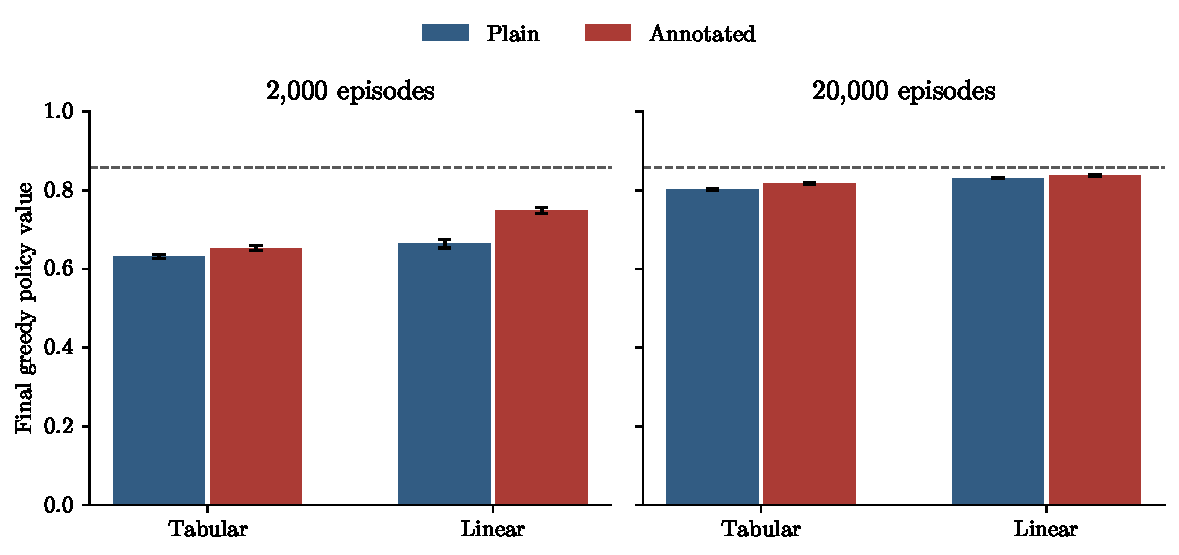
\includegraphics[width=0.95\linewidth,height=\textheight,keepaspectratio,alt={Final greedy values at two retained training horizons. Error bars are the record's standard errors across 30 seeds, not confidence intervals or a test of the paired difference. The dashed line is the enumerated joint optimum.}]{figures/final-values.pdf}
\caption{Final greedy values at two retained training horizons. Error
bars are the record's standard errors across 30 seeds, not confidence
intervals or a test of the paired difference. The dashed line is the
enumerated joint optimum.}
\end{figure}

The linear learner uses context/action and flag/action features. The
annotated version adds the shared indicator \(\mathbf1[a=c]\). This
changes the available feature list, so its finite-horizon gains cannot
be interpreted solely as an effect on an otherwise identical
representation. The saved record also includes constant-step tabular and
sampled-query variants. No new training runs were performed for this
paper.

\section{7. Remaining questions}\label{remaining-questions}

A learning-rate theorem needs an explicit learner, feature class,
context distribution, accuracy target and confidence level. An assertion
of constant versus context-linear sample complexity cannot be assessed
without those inputs. The simulations provide finite-horizon
comparisons, not such a theorem.

Theorems 2 and 4 also answer different questions. The first values
private information under a fixed query distribution. The second follows
a specified learning process whose greedy query eventually stabilizes.
Neither establishes a universal advantage for the SelfRefl wrapper over
all agents, and neither is a theorem about general policy-dependent
MDPs.

The principal lesson for a proposed formal performance claim is to
specify the query/action coupling, accessible information, policy class,
training updates and evaluation objective together. The proofs and
examples above make those choices inspectable.

\section{References}\label{references}

\textbf{{[}A{]}} Samuel Allen Alexander. \emph{Pseudo-visibility: a game
mechanic involving willful ignorance}. Proceedings of FLAIRS-35 (2022).
\href{https://doi.org/10.32473/flairs.v35i.130652}{DOI:
10.32473/flairs.v35i.130652}. Definitions 2 and 9--10, discussion after
Lemma 4, Proposition 12, and the concluding better-performance
discussion.

\end{document}
